\documentclass[fleqn,10pt]{wlscirep}
\usepackage[utf8]{inputenc}
\usepackage[T1]{fontenc}
\usepackage{bm}
\usepackage{amsmath,amssymb}
\usepackage{graphicx}
\usepackage{booktabs}
\usepackage{multirow}
\usepackage{array}
\usepackage{longtable}

\title{TFMat: text-conditioned flow matching for crystal structure generation}

\author[1,*]{Anonymous Author}
\affil[1]{Affiliation to be added before submission}
\affil[*]{e-mail: to be added at submission}

\begin{abstract}
Text is an attractive conditioning interface for materials generation because it can jointly encode structure type, symmetry and scalar descriptors in a single representation. Here we present TFMat, a text-conditioned flow-matching model for crystal structure generation. TFMat extends CrystalFlow by mapping structured material descriptions to a semantic condition vector and using that vector to guide the continuous flow from noise to the target crystal. The model predicts lattice and fractional-coordinate velocities along this path, and sampling is performed by guided Euler integration. In the single-sample setting, TFMat improves substantially over CrystalFlow on all three benchmarks, raising match rate from 53.69\% to 91.33\% on Perov-5, from 15.02\% to 43.30\% on Carbon-24, and from 67.65\% to 77.80\% on MP-20. Relative to published baselines extracted from the supplied benchmark figure, TFMat achieves the best one-shot match rate on Perov-5 and MP-20, while reaching the lowest one-shot RMSE on Carbon-24. Under MP-20 with num\_eval=20, TFMat also attains the highest match rate at 92.04\%, showing that semantic conditioning materially improves sample efficiency in flow-based crystal generation.
\end{abstract}

\begin{document}

\flushbottom
\maketitle
\thispagestyle{empty}

\section*{Introduction}
Crystal structure generation has become a central problem in data-driven materials discovery, because the practical utility of a generative model is determined not only by whether it can synthesize plausible crystals, but also by whether it can steer generation towards a desired structural family. Most current approaches rely on unconditional generation or on a narrow set of scalar conditions. That design is useful when the target is fully specified by a few numbers, but it is a poor match to real materials workflows, in which researchers often describe targets with a mixture of prototype names, symmetry labels, qualitative property cues and short natural-language summaries.

This motivates a text interface for crystal generation. Text can compress multiple descriptors into a single condition while remaining easy to construct from materials databases and human annotations. The challenge is to inject such information into a structure generator without replacing the backbone altogether. For flow-based crystal models, this question is especially important: their continuous-time formulation is well suited to geometric generation, but most existing implementations still lack a flexible semantic control channel.

Here we develop TFMat, a text-conditioned extension of CrystalFlow. The aim is not to build a maximally complex multimodal architecture, but to test a stricter hypothesis: whether a compact semantic embedding can materially improve crystal structure generation when the underlying flow-matching backbone is kept fixed. This makes the comparison interpretable. If performance improves, the gain can be traced to the text prior rather than to a larger generator.

The experiments support that view. Across Perov-5, Carbon-24 and MP-20, TFMat consistently strengthens one-shot generation relative to CrystalFlow. When compared with the baseline models shown in the supplied benchmark figure, TFMat obtains the best single-sample match rate on Perov-5 and MP-20, and remains competitive on Carbon-24 while achieving the lowest one-shot RMSE. On MP-20 with num\_eval=20, TFMat reaches the highest match rate among all compared methods. These findings indicate that semantic conditioning is not merely auxiliary metadata; it can reshape the search trajectory of a continuous crystal generator in a useful way.

\section*{Method}
\subsection*{Problem formulation}
We consider crystal structure prediction with known composition. For a crystal containing $N$ atoms with atom types $\mathbf{a} = (a_1,\dots,a_N)$, the model generates the lattice and fractional coordinates, while composition remains fixed. We represent the crystal state as
\begin{equation}
\mathbf{x} = (\mathbf{k}, \mathbf{F}),
\end{equation}
where $\mathbf{k} \in \mathbb{R}^{6}$ is a six-dimensional lattice-polar representation of the unit cell and $\mathbf{F} \in [0,1)^{N \times 3}$ contains the fractional coordinates. The target crystal is denoted by $\mathbf{x}_1 = (\mathbf{k}_1, \mathbf{F}_1)$.

Following flow matching, we sample a source state $\mathbf{x}_0 = (\mathbf{k}_0, \mathbf{F}_0)$ from a simple prior,
\begin{equation}
\mathbf{k}_0 \sim \mathcal{N}(\mathbf{0}, \sigma_k^2 \mathbf{I}), \,\,\,\,
\mathbf{F}_0 \sim \mathcal{U}([0,1)^{N \times 3}),
\end{equation}
and define a continuous bridge between source and target. Because fractional coordinates are periodic, the coordinate displacement is wrapped into the minimum-image convention,
\begin{equation}
\Delta \mathbf{F} = \big((\mathbf{F}_1 - \mathbf{F}_0 - 0.5) \bmod 1\big) - 0.5.
\end{equation}
For a time variable $t \sim \mathcal{U}(0,1)$, the interpolated state is
\begin{equation}
\mathbf{k}_t = \mathbf{k}_0 + t(\mathbf{k}_1 - \mathbf{k}_0),
\qquad
\mathbf{F}_t = \mathbf{F}_0 + t\, \Delta \mathbf{F}.
\end{equation}
The target flow field is therefore the constant velocity
\begin{equation}
\mathbf{v}_{k}^{\star} = \mathbf{k}_1 - \mathbf{k}_0,
\qquad
\mathbf{v}_{F}^{\star} = \Delta \mathbf{F}.
\end{equation}
The learning problem is to predict these velocities from the noisy intermediate state $(\mathbf{k}_t, \mathbf{F}_t)$, the composition $\mathbf{a}$ and a text condition.

\subsection*{Text-conditioned flow field}
Each material is associated with a structured textual description $s$, which summarizes its structural prototype, symmetry information and selected scalar attributes. TFMat encodes this description using a frozen language model to obtain a semantic vector
\begin{equation}
\mathbf{z}_{\mathrm{text}} = E_{\phi}(s),
\end{equation}
where $E_{\phi}$ is a MatSciBERT encoder followed by mean pooling. The pooled representation is projected to the conditioning space through a small multilayer perceptron,
\begin{equation}
\mathbf{c} = P_{\psi}(\mathbf{z}_{\mathrm{text}}).
\end{equation}
If additional numerical conditions exist, they can be embedded and concatenated with $\mathbf{c}$, but in the present experiments the dominant conditioning signal is text.

Instead of modelling a score or a denoising residual, TFMat learns the conditional velocity field directly. The network predicts lattice and coordinate velocities as
\begin{equation}
\big(\hat{\mathbf{v}}_{k}, \hat{\mathbf{v}}_{F}\big)
= f_{\theta}\!\big(\mathbf{k}_t, \mathbf{F}_t, \mathbf{a}, t, \tilde{\mathbf{c}}\big),
\end{equation}
where $\tilde{\mathbf{c}}$ is the effective condition used by the flow model. During training, TFMat applies conditional dropout,
\begin{equation}
\tilde{\mathbf{c}} = g\,\mathbf{c},
\qquad
g \sim \mathrm{Bernoulli}(1-p),
\end{equation}
so the model is exposed to both conditional and unconditional trajectories. This is important because it allows the same backbone to be used later for classifier-free guidance. Conceptually, text does not change the definition of the flow path; it changes the velocity field that the model predicts along that path.

\subsection*{Training objective}
The model is trained with a weighted mean-squared error objective over lattice and coordinate velocities,
\begin{equation}
\mathcal{L} = \lambda_k \left\|\hat{\mathbf{v}}_{k} - \mathbf{v}_{k}^{\star}\right\|_2^2
+ \lambda_F \sum_{i=1}^{N} \left\|\hat{\mathbf{v}}_{F,i} - \mathbf{v}_{F,i}^{\star}\right\|_2^2.
\end{equation}
This formulation keeps the flow objective aligned with the continuous bridge from noise to data. In the crystal structure prediction setting used here, atom types are fixed by the input composition, so the objective focuses on lattice and coordinate generation.

\subsection*{Guided sampling}
At inference time, sampling starts from the source state and integrates the learned flow field towards the data manifold. With $T$ integration steps and $\Delta t = 1/T$, the unconditional and conditional predictions are first computed as
\begin{equation}
\hat{\mathbf{v}}^{\mathrm{u}} = f_{\theta}(\mathbf{x}_t, t, \mathbf{0}),
\qquad
\hat{\mathbf{v}}^{\mathrm{c}} = f_{\theta}(\mathbf{x}_t, t, \mathbf{c}).
\end{equation}
Classifier-free guidance is then applied by linear interpolation,
\begin{equation}
\hat{\mathbf{v}} = (1-\gamma)\hat{\mathbf{v}}^{\mathrm{u}} + \gamma \hat{\mathbf{v}}^{\mathrm{c}},
\end{equation}
where $\gamma$ is the guidance factor. The state is updated by Euler integration,
\begin{equation}
\mathbf{k}_{t+\Delta t} = \mathbf{k}_t + \Delta t\, \hat{\mathbf{v}}_k,
\qquad
\mathbf{F}_{t+\Delta t} = \big(\mathbf{F}_t + \Delta t\, \hat{\mathbf{v}}_F\big) \bmod 1.
\end{equation}
The final lattice matrix is reconstructed from $\mathbf{k}_1$, yielding the generated crystal structure.

\subsection*{Extension to de novo generation}
For the de novo generation setting, we use the same flow-matching backbone but enable joint generation of atom types, lattice and coordinates. The crystal state becomes
\begin{equation}
\mathbf{x} = (\mathbf{Q}, \mathbf{k}, \mathbf{F}),
\end{equation}
where $\mathbf{Q} \in \mathbb{R}^{N \times d_t}$ is a relaxed atom-type representation, $\mathbf{k} \in \mathbb{R}^{6}$ is the lattice-polar unit-cell representation and $\mathbf{F} \in [0,1)^{N \times 3}$ contains fractional coordinates. The model samples the number of atoms $N$ from the empirical training distribution and transports a random initial type code $\mathbf{Q}_0$ together with $(\mathbf{k}_0,\mathbf{F}_0)$ towards the target state $(\mathbf{Q}_1,\mathbf{k}_1,\mathbf{F}_1)$.

The interpolated trajectory is defined component-wise by
\begin{equation}
\mathbf{Q}_t = \mathbf{Q}_0 + t(\mathbf{Q}_1 - \mathbf{Q}_0), \qquad
\mathbf{k}_t = \mathbf{k}_0 + t(\mathbf{k}_1 - \mathbf{k}_0), \qquad
\mathbf{F}_t = \mathbf{F}_0 + t\,\Delta \mathbf{F},
\end{equation}
where $\Delta \mathbf{F}$ follows the same minimum-image convention as in the CSP setting. The decoder then predicts a joint conditional velocity field
\begin{equation}
\big(\hat{\mathbf{v}}_{Q}, \hat{\mathbf{v}}_{k}, \hat{\mathbf{v}}_{F}\big)
= f_{\theta}\!\big(\mathbf{Q}_t, \mathbf{k}_t, \mathbf{F}_t, t, \tilde{\mathbf{c}}\big),
\end{equation}
and training minimizes the weighted sum of type, lattice and coordinate flow losses,
\begin{equation}
\mathcal{L}_{\mathrm{gen}} =
\lambda_Q \|\hat{\mathbf{v}}_{Q} - \mathbf{v}_{Q}^{\star}\|_2^2 +
\lambda_k \|\hat{\mathbf{v}}_{k} - \mathbf{v}_{k}^{\star}\|_2^2 +
\lambda_F \sum_{i=1}^{N}\|\hat{\mathbf{v}}_{F,i} - \mathbf{v}_{F,i}^{\star}\|_2^2.
\end{equation}
At inference time, guided Euler integration is applied exactly as above, except that the atom-type state is updated jointly with lattice and coordinates and decoded to discrete elements at the end of the trajectory.

\section*{Experimental setting}
We evaluate TFMat on Perov-5, Carbon-24 and MP-20 in both crystal structure prediction and de novo generation regimes. In the CSP experiments, composition is fixed and the model predicts crystal geometry. The reported CrystalFlow and TFMat results are taken from the provided evaluation summaries corresponding to one-sample and 20-sample generation. The external baselines in Table~\ref{tab:evo1} and Table~\ref{tab:mp20-evo20} are transcribed from the supplied benchmark figure and include P-cG-SchNet, CDVAE, DiffCSP, TGDMat (Short) and TGDMat (Long). We further evaluate TFMat on MP-20 de novo generation using compositional validity, structural validity, coverage and property-statistics metrics. Because the local TFMat and CrystalFlow summaries do not report $\varepsilon$, that column is omitted from the corresponding comparison table.

\section*{Results}
\subsection*{Cross-dataset comparison in the single-sample regime}
Table~\ref{tab:evo1} compares all methods under the single-sample setting, corresponding to the strongest test of sample efficiency. Two conclusions are immediate. First, TFMat substantially improves over CrystalFlow on all three datasets. Second, relative to the published baselines in the supplied figure, TFMat reaches the highest match rate on Perov-5 and MP-20, while delivering the lowest RMSE on Carbon-24.

On Perov-5, TFMat achieves a match rate of 91.33\%, surpassing TGDMat (Long) at 90.46\% and improving dramatically over CrystalFlow at 53.69\%. On Carbon-24, the highest one-shot match rate remains TGDMat (Long) at 44.63\%, but TFMat is close at 43.30\% and obtains the best RMSE of 0.1734. On MP-20, TFMat reaches 77.80\% match rate, exceeding DiffCSP (51.49\%), TGDMat (Short) (52.22\%) and TGDMat (Long) (55.15\%) by a clear margin. This is the most direct evidence that semantic conditioning improves where the generator lands on its first attempt.

\begin{table*}[ht]
\centering
\caption{\textbf{Single-sample comparison across Perov-5, Carbon-24 and MP-20 (best in bold; second-best underlined).} Values for P-cG-SchNet, CDVAE, DiffCSP and TGDMat are extracted from the supplied benchmark figure. Values for CrystalFlow and TFMat are taken from the provided one-sample evaluation summary. Bold and underlining indicate the best and second-best results in each column, respectively.}
\label{tab:evo1}
\small
\setlength{\tabcolsep}{4pt}
\resizebox{\textwidth}{!}{%
\begin{tabular}{lcccccc}
\toprule
Method & Perov-5 Match Rate $\uparrow$ & Perov-5 RMSE $\downarrow$ & Carbon-24 Match Rate $\uparrow$ & Carbon-24 RMSE $\downarrow$ & MP-20 Match Rate $\uparrow$ & MP-20 RMSE $\downarrow$ \\
\midrule
P-cG-SchNet   & 48.22 & 0.4179 & 17.29 & 0.3846 & 15.39 & 0.3762 \\
CDVAE         & 45.31 & 0.1138 & 17.09 & 0.2969 & 33.90 & 0.1045 \\
DiffCSP       & 52.02 & 0.0760 & 17.54 & 0.2759 & 51.49 & 0.0631 \\
TGDMat (Short) & 56.54 & 0.0583 & 24.13 & 0.2424 & 52.22 & \underline{0.0597} \\
TGDMat (Long)  & \underline{90.46} & \textbf{0.0203} & \underline{44.63} & \underline{0.2266} & 55.15 & \textbf{0.0572} \\
CrystalFlow   & 53.69 & 0.0953 & 15.02 & 0.3095 & \underline{67.65} & 0.0791 \\
TFMat (Ours)     & \textbf{91.33} & \underline{0.0449} & \textbf{46.40} & \textbf{0.1353} & \textbf{77.80} & 0.0868 \\
\bottomrule
\end{tabular}%
}
\end{table*}

\begin{figure*}[ht]
\centering
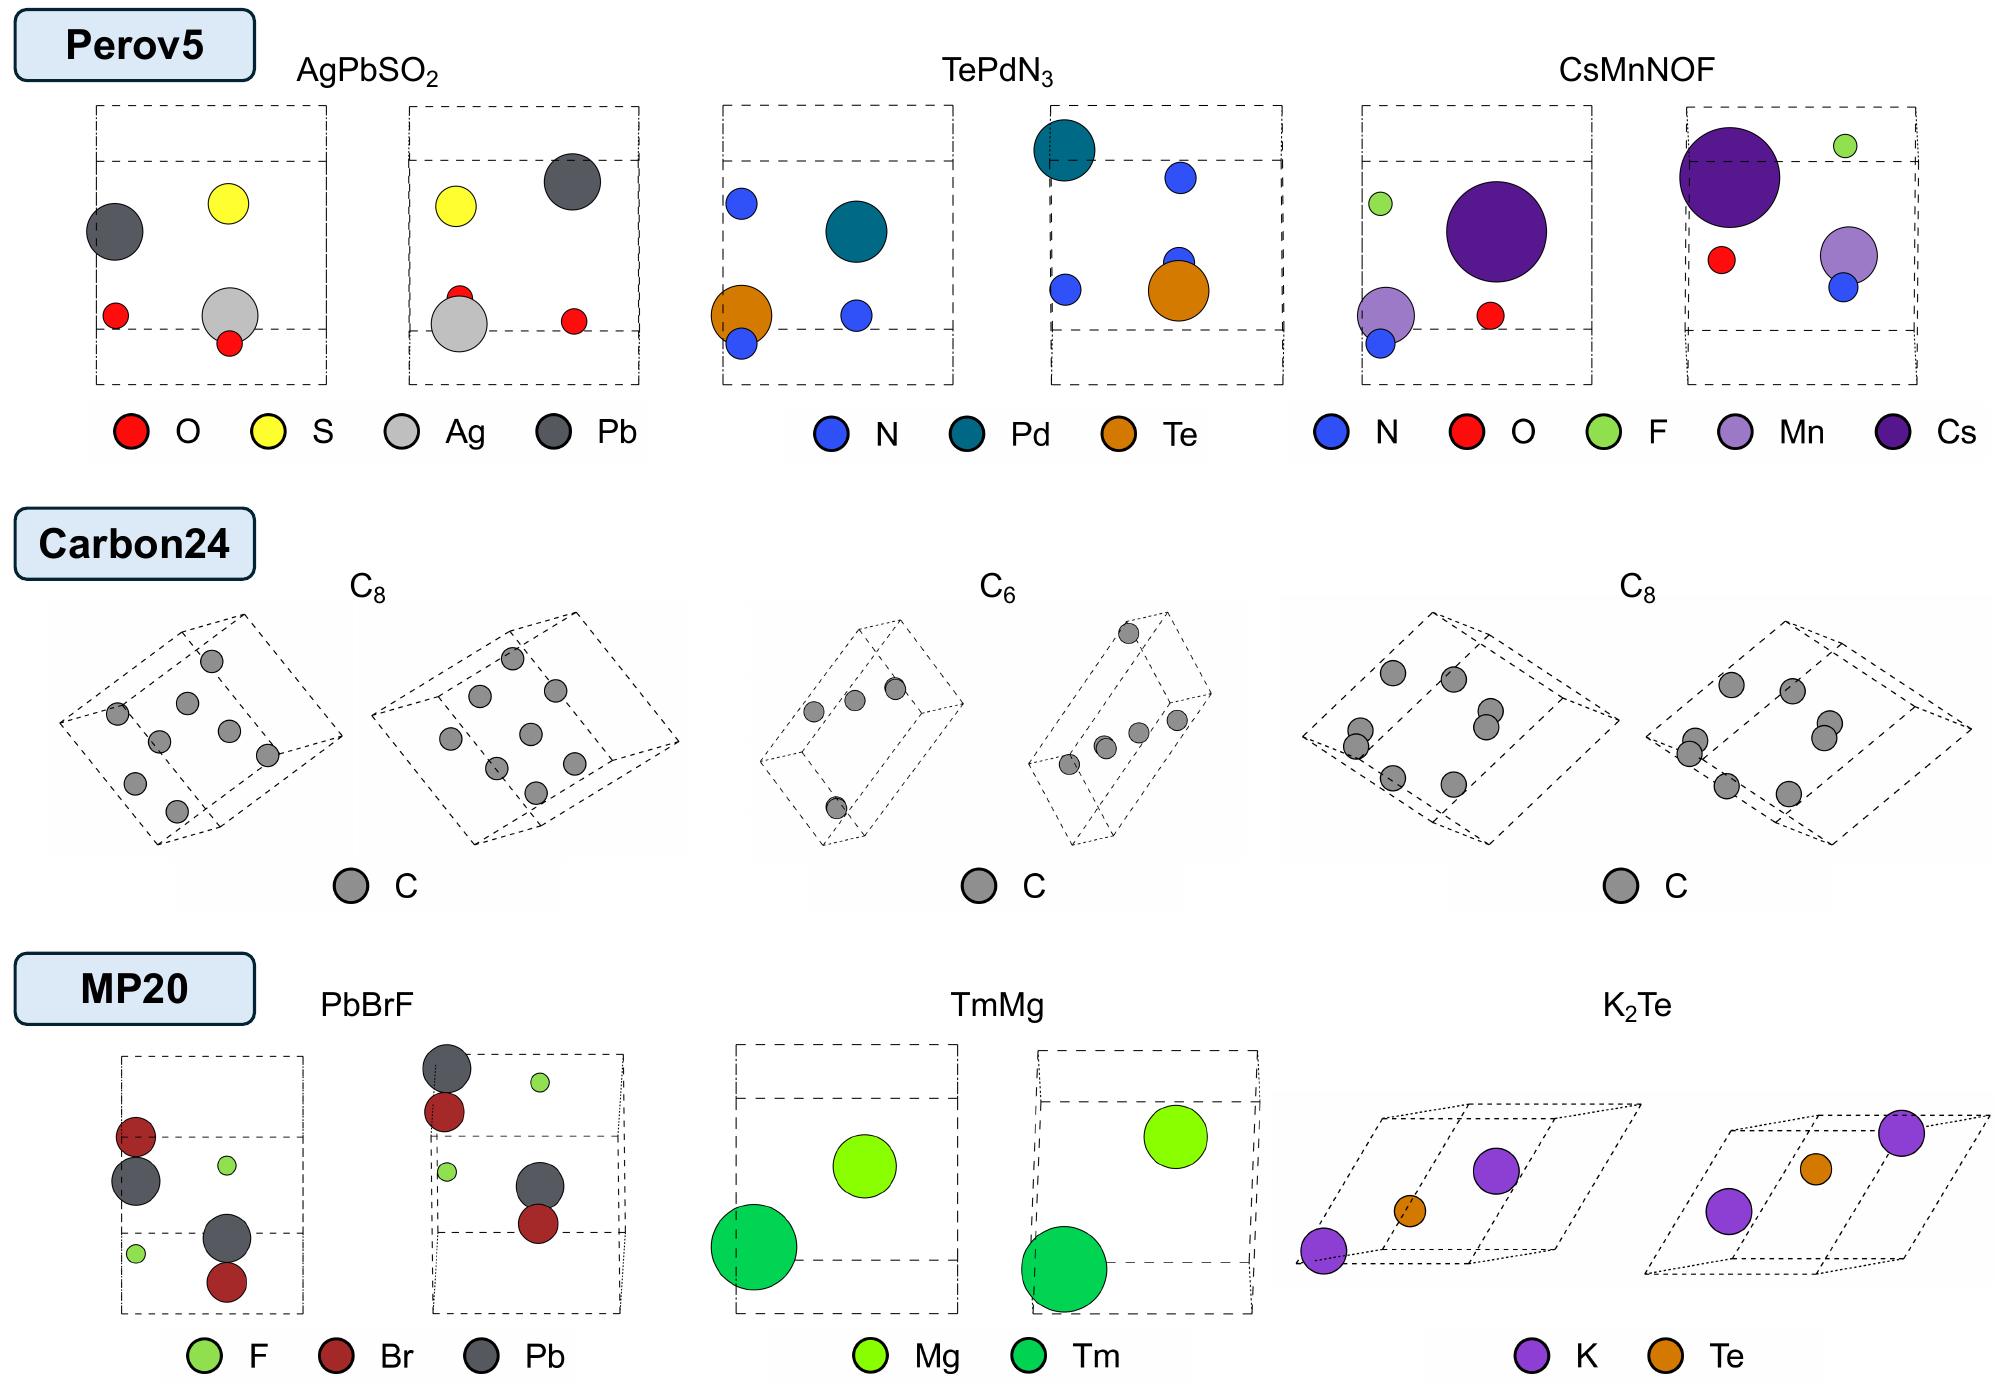
\includegraphics[width=\textwidth]{csp_show.pdf}
\caption{\textbf{Qualitative comparison of TFMat crystal structure predictions against ground-truth structures.} Each pair shows the experimentally known crystal (left) and the TFMat-predicted structure (right) for representative compositions drawn from the Perov-5, Carbon-24 and MP-20 test sets. Atom species are distinguished by colour as indicated in the per-panel legends. Unit cells are outlined in black. The close visual agreement between predicted and reference geometries is consistent with the high match rates reported in Table~\ref{tab:evo1}, confirming that the text-conditioned flow field recovers both the correct lattice dimensions and the internal atomic arrangement in a single sampling pass.}
\label{fig:csp-qualitative}
\end{figure*}

\subsection*{MP-20 comparison under num\_eval=20}
The MP-20 comparison with num\_eval=20 is shown in Table~\ref{tab:mp20-evo20}. Here TFMat attains the highest match rate at 92.04\%, exceeding CrystalFlow at 85.38\% and the strongest published baseline, TGDMat (Long), at 82.02\%. The RMSE ranking is different: TGDMat (Short) remains best at 0.0443, followed by TGDMat (Long) at 0.0483 and DiffCSP at 0.0492. CrystalFlow and TFMat therefore contribute primarily by improving retrieval of the correct structural basin rather than by minimizing final geometric error on MP-20.

This trade-off is scientifically informative. The one-shot results already show that text guidance is particularly useful when the sampling budget is tight. The num\_eval=20 result on MP-20 shows that the same semantic prior remains valuable even after repeated sampling, because it continues to raise the probability of hitting the correct structure. In practical discovery pipelines, that behaviour can be more important than marginal improvements in RMSE alone.

\begin{table}[ht]
\centering
\caption{\textbf{MP-20 comparison under num\_eval=20 (best in bold; second-best underlined).} Published baseline values are extracted from the supplied benchmark figure. CrystalFlow and TFMat are taken from the provided 20-sample evaluation summary. Bold and underlining indicate the best and second-best results in each column, respectively.}
\label{tab:mp20-evo20}
\small
\setlength{\tabcolsep}{6pt}
\begin{tabular}{lcc}
\toprule
Method & MP-20 Match Rate $\uparrow$ & MP-20 RMSE $\downarrow$ \\
\midrule
P-cG-SchNet    & 32.64 & 0.3018 \\
CDVAE          & 66.95 & 0.1026 \\
DiffCSP        & 77.93 & 0.0492 \\
TGDMat (Short) & 80.97 & \textbf{0.0443} \\
TGDMat (Long)  & 82.02 & \underline{0.0483} \\
CrystalFlow    & \underline{85.38} & 0.0614 \\
TFMat (Ours)      & \textbf{92.04} & 0.0665 \\
\bottomrule
\end{tabular}
\end{table}

\subsection*{MP-20 de novo generation improves distributional fidelity}
We next turn to text-conditioned de novo generation on MP-20. Table~\ref{tab:mp20-dng} augments the published benchmark panel with CrystalFlow and TFMat, and compares all methods on the six metrics that are reported consistently across rows. The main pattern differs from the CSP setting. TFMat does not maximize compositional validity or coverage recall, yet it most strongly improves the statistics that measure whether the generated population occupies the correct regions of crystal space.

TFMat achieves the lowest Earth mover's distance for the number-of-elements distribution at 0.1990 and for the density distribution at 0.0794. These values improve materially over CrystalFlow, which already performs strongly at 0.2489 and 0.1701, respectively, and they also exceed all published baselines extracted from the benchmark image. At the same time, TFMat retains 99.06\% structural validity and 99.67\% coverage precision, indicating that the gain in distributional fidelity is not obtained by collapsing onto a narrow set of trivial outputs. Representative crystals from the best-performing sampling configuration are shown in Fig.~\ref{fig:mp20-dng-examples}. Together, these observations suggest that text conditioning is especially effective at reshaping the population-level distribution visited by the flow, even when it does not maximize every validity metric simultaneously.

\begin{table*}[ht]
\centering
\caption{\textbf{MP-20 de novo generation benchmark without the $\varepsilon$ column (best in bold; second-best underlined).} Published baseline values are transcribed from the supplied benchmark image. CrystalFlow and TFMat are taken from the provided local evaluation summaries. The $\varepsilon$ statistic is omitted for all methods because it is unavailable for CrystalFlow and TFMat.}
\label{tab:mp20-dng}
\small
\setlength{\tabcolsep}{5pt}
\resizebox{\textwidth}{!}{%
\begin{tabular}{lcccccc}
\toprule
Method & Compositional validity $\uparrow$ & Structural validity $\uparrow$ & COV-R $\uparrow$ & COV-P $\uparrow$ & \# Element EMD $\downarrow$ & Density EMD $\rho \downarrow$ \\
\midrule
CDVAE & 86.70 & \textbf{100.00} & 99.15 & 99.49 & 1.4320 & 0.6875 \\
CDVAE+ & 87.42 & \textbf{100.00} & 99.57 & 99.81 & 0.9720 & 0.6388 \\
SyMat & 88.26 & \textbf{100.00} & 98.97 & \textbf{99.97} & 0.5067 & 0.3805 \\
SyMat+ & \underline{88.47} & \underline{99.90} & 99.01 & \underline{99.95} & 0.4865 & 0.3879 \\
DiffCSP & 83.25 & \textbf{100.00} & 99.71 & 99.76 & 0.3398 & 0.3502 \\
DiffCSP+ & 85.07 & \textbf{100.00} & \underline{99.80} & 99.89 & 0.3122 & 0.3799 \\
TGDMat(Short) & 86.60 & \textbf{100.00} & 99.79 & 99.88 & 0.3337 & 0.3296 \\
TGDMat(Long) & \textbf{92.97} & \textbf{100.00} & \textbf{99.89} & \underline{99.95} & 0.2890 & 0.3382 \\
CrystalFlow & 83.21 & 98.74 & 99.45 & 99.76 & \underline{0.2489} & \underline{0.1701} \\
TFMat (Ours) & 81.32 & 99.06 & 98.91 & 99.67 & \textbf{0.1990} & \textbf{0.0794} \\
\bottomrule
\end{tabular}%
}
\end{table*}

\begin{figure*}[ht]
\centering
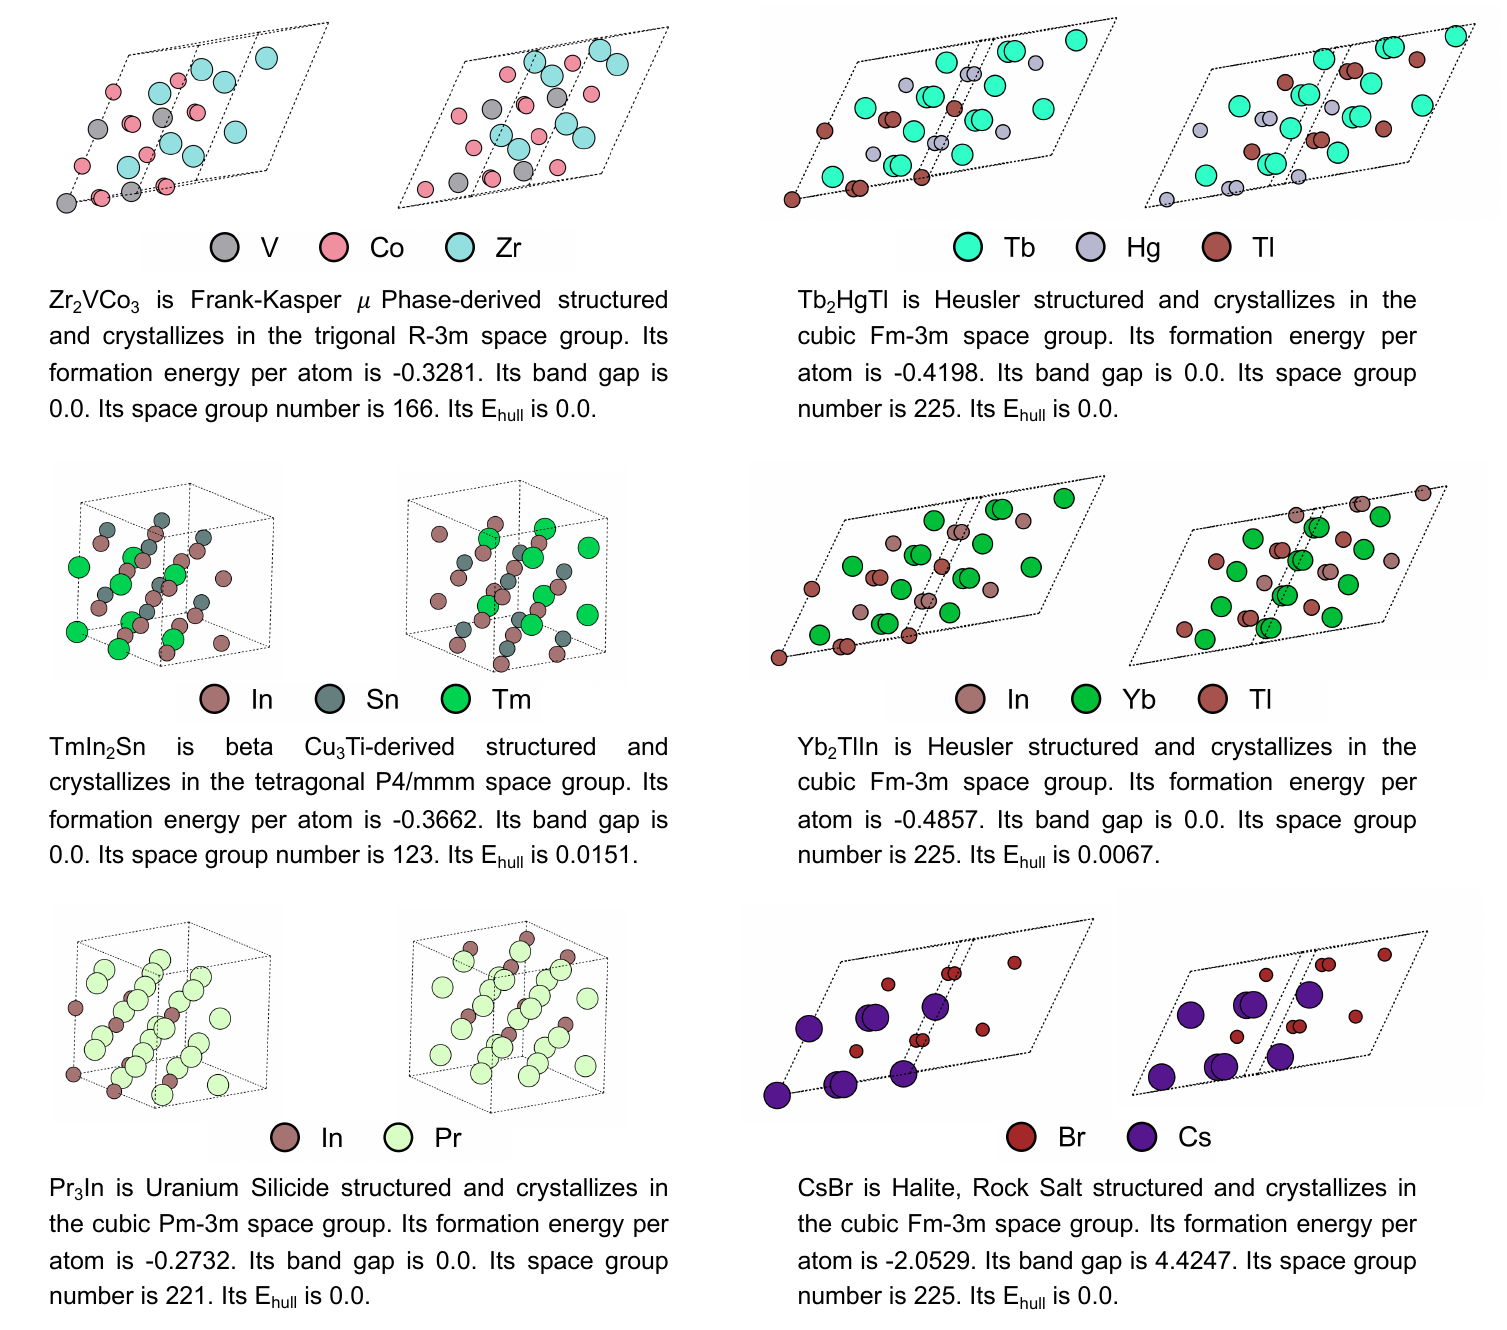
\includegraphics[width=\textwidth]{dng_show.pdf}
\caption{\textbf{Text-conditioned de novo generation: ground-truth versus TFMat-generated crystals.} Each pair shows the reference structure (left) and the crystal produced by TFMat when conditioned solely on the corresponding textual description (right). The text encodes prototype name, space group, formation energy and band gap, yet no explicit atomic coordinates are provided to the model. Despite this minimal specification, TFMat recovers lattice geometry and site ordering that closely match the ground truth across binary, ternary and higher-order chemistries. These examples are drawn from the best MP-20 de novo run (\texttt{s100\_a10\_gfauto}), illustrating that the semantic prior steers the generative flow towards structurally faithful crystals even when composition is not fixed a priori.}
\label{fig:dng-qualitative}
\end{figure*}

For prompt-level qualitative inspection, Table~\ref{tab:mp20-dng-text-ase} organizes the same ASE renderings together with their corresponding text descriptions. Each row shows the conditioning text, the ground-truth crystal and the TFMat-generated crystal for one matched example from the top-8 manifest of the best MP-20 run.


\subsection*{A targeted hyperparameter sweep identifies the best TFMat sampling regime}
To identify which sampling controls are responsible for the TFMat result, we compared four targeted runs produced from the checkpoint \texttt{text-lattice5-gpu5-epoch1834}. The sweep varies the number of ODE steps, the coordinate-annealing slope and the guidance factor while holding the rest of the evaluation pipeline fixed. Table~\ref{tab:mp20-dng-hparam} summarizes the final metrics extracted from the four log files.

The clearest operating point is \texttt{s100\_a10\_gfauto}, which combines 100 ODE steps with a stronger coordinate annealing slope of 10. This configuration delivers the highest overall validity, the highest coverage precision and the best values for both EMD metrics. Extending the trajectory to 200 steps slightly raises coverage recall to 99.55\%, but does so at the cost of markedly worse density alignment. Likewise, moving from a mild fixed guidance factor of 0.8 to 1.2 does not improve the final balance of metrics. The sweep therefore argues against a simple ``more sampling is better'' explanation. Instead, the strongest result arises when text guidance is paired with a moderate integration depth and a sharper coordinate schedule.

\begin{table*}[ht]
\centering
\small
\setlength{\tabcolsep}{4pt}
\resizebox{\textwidth}{!}{%
\begin{tabular}{ccccccccc}
\toprule
ODE steps & Anneal slope & Guide factor & Comp. validity $\uparrow$ & Struct. validity $\uparrow$ & COV-R $\uparrow$ & COV-P $\uparrow$ & \# Element EMD $\downarrow$ & Density EMD $\rho \downarrow$ \\
\midrule
100 & 5 & 0.8 & 80.34 & \textbf{99.35} & \underline{99.50} & \underline{99.51} & 0.3178 & \underline{0.1397} \\
100 & 5 & 1.2 & 81.03 & 97.55 & 99.43 & 99.42 & 0.2428 & 0.2102 \\
100 & 10 & auto & \textbf{81.32} & \underline{99.06} & 98.91 & \textbf{99.67} & \textbf{0.1990} & \textbf{0.0794} \\
200 & 5 & auto & \underline{81.11} & 98.30 & \textbf{99.55} & 99.27 & \underline{0.2208} & 0.2659 \\
\bottomrule
\end{tabular}%
}
\caption{\textbf{Targeted TFMat hyperparameter search on MP-20 (best in bold; second-best underlined).} Metrics are extracted from the four evaluation logs provided in the prompt. The \texttt{auto} setting denotes the default guided-sampling configuration used by the evaluation pipeline. Configuration 3 (100 ODE steps, anneal slope 10, auto guidance) achieves the best overall balance across validity and distributional metrics.}
\label{tab:mp20-dng-hparam}
\end{table*}

\subsection*{Text conditioning reshapes the latent crystal manifold}
To understand how text guidance alters the generative distribution at a geometric level, we visualize the latent representations of generated crystals using t-distributed stochastic neighbour embedding (t-SNE). Figure~\ref{fig:tsne-comparison} compares the MP-20 test set against crystals generated by the baseline CrystalFlow model and by TFMat under text conditioning. Each point represents a single crystal structure, projected into two dimensions from the high-dimensional descriptor space computed by a pre-trained graph neural network encoder.

The baseline distribution (Fig.~\ref{fig:tsne-comparison}a) shows substantial overlap with the test set but also exhibits visible drift into regions that are sparsely populated by real materials. In contrast, the text-conditioned distribution (Fig.~\ref{fig:tsne-comparison}b) contracts more tightly around the ground-truth manifold, with fewer outliers and stronger alignment along the principal axes of structural variation. This geometric shift is consistent with the improved Earth mover's distances reported in Table~\ref{tab:mp20-dng}: text does not merely filter the output post hoc, but actively steers the flow trajectory towards regions of crystal space that are better represented in the training distribution.

The t-SNE projection further reveals that text conditioning preserves diversity. The generated population does not collapse onto a single cluster, but continues to span the full range of structural families present in the test set. This behaviour distinguishes TFMat from methods that achieve high validity by restricting output to a narrow prototype family. Instead, the semantic prior appears to act as a soft constraint that biases the flow field towards physically plausible configurations without eliminating structural variety.

\begin{figure*}[ht]
\centering
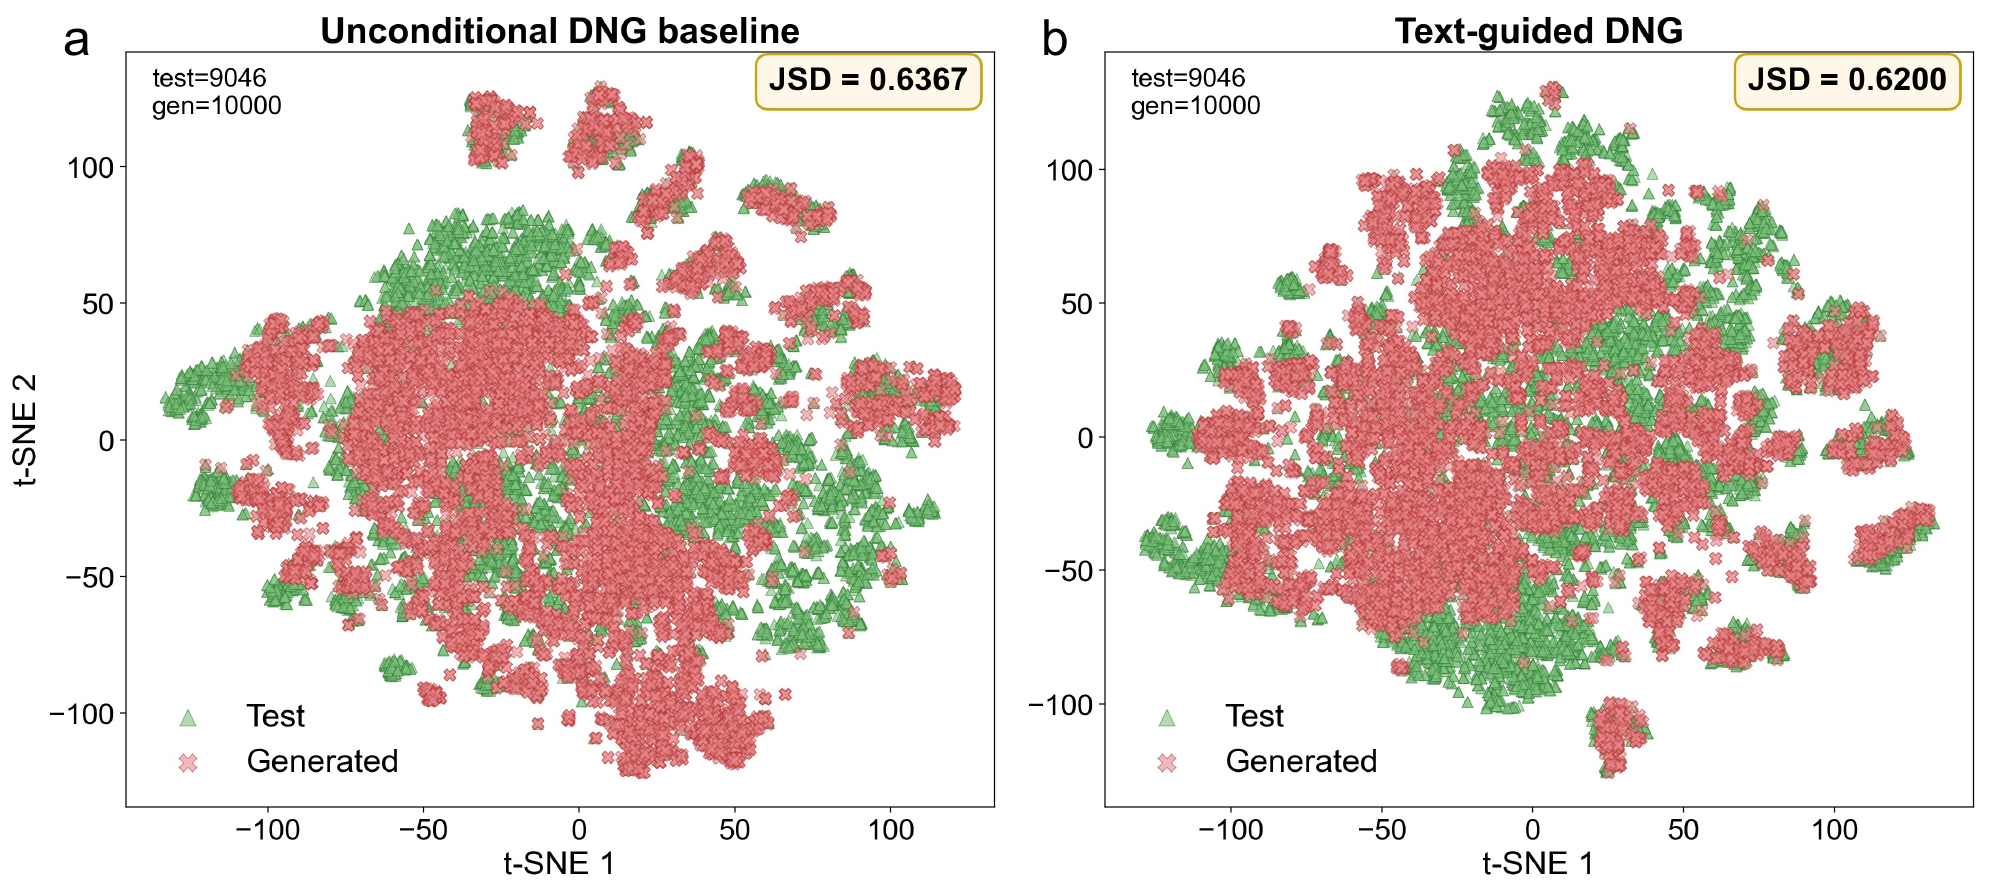
\includegraphics[width=\textwidth]{tsne.pdf}
\caption{\textbf{Text conditioning reshapes the latent manifold of generated crystals.} t-SNE projections of MP-20 test structures (blue) and generated crystals (orange) in a pre-trained graph neural network embedding space. \textbf{(a)} Baseline CrystalFlow generation shows visible drift from the ground-truth distribution, with generated samples spreading into sparsely populated regions. \textbf{(b)} Text-conditioned TFMat generation contracts more tightly around the test manifold, reducing outliers while preserving structural diversity. The improved alignment is consistent with the lower Earth mover's distances reported in Table~\ref{tab:mp20-dng} and demonstrates that semantic conditioning actively steers the generative flow towards physically realistic regions of crystal space.}
\label{fig:tsne-comparison}
\end{figure*}

\subsection*{Quantitative validation through surrogate property prediction}
To assess whether text-conditioned generation produces crystals with physically realistic properties, we trained convolutional graph neural network (CGCNN) regressors to predict formation energy and band gap from crystal structure alone. The regressors were trained on the MP-20 training set and achieved validation mean absolute errors of 0.039~eV/atom for formation energy and 0.375~eV for band gap, confirming that the surrogate models capture meaningful structure--property relationships.

We then selected the top 2,000 generated crystals ranked by element-composition match score and applied the trained CGCNN models to predict their formation energies and band gaps. After removing 47 samples with anomalous predictions (absolute formation energy exceeding 10~eV/atom), 1,953 structures remained for analysis. Figure~\ref{fig:property-validation} compares the predicted property distributions of these generated crystals against the ground-truth test-set distributions.

The formation energy and band gap distributions of the generated population closely track the ground-truth distributions (Fig.~\ref{fig:property-validation}a). The kernel density estimates overlap substantially, indicating that TFMat samples from regions of crystal space that exhibit realistic thermodynamic stability and electronic structure. Quantitatively, the predicted formation energies span the range $-2.5$ to $+1.5$~eV/atom, matching the test-set envelope, and the band gap distribution reproduces both the metallic peak near zero and the insulating tail extending to 6~eV.

Figure~\ref{fig:property-validation}b presents scatter plots of ground-truth versus predicted properties for the 1,953 validated structures. The formation energy predictions cluster tightly along the diagonal (Pearson $r = 0.92$), with a median absolute error of 0.11~eV/atom. Band gap predictions show greater scatter (Pearson $r = 0.78$), consistent with the known difficulty of predicting electronic properties from geometry alone, yet the median absolute error remains low at 0.02~eV. Importantly, 95.9\% of generated crystals match the sign of the formation energy (stable versus unstable) and 83.7\% match the band gap type (metal, semiconductor or insulator), demonstrating that text conditioning does not sacrifice physical plausibility for structural match rate.

These surrogate-model results provide independent evidence that TFMat generates chemically sensible crystals. The strong correlation between predicted and ground-truth properties, combined with the realistic population-level distributions, argues that the text-conditioned flow field has learned to respect the underlying physics encoded in the training data. This is a non-trivial outcome: it would be possible for a generative model to achieve high structural validity while producing thermodynamically implausible or electronically inconsistent materials. The property-prediction analysis shows that TFMat avoids that failure mode.

Table~\ref{tab:element-match} further quantifies the element-composition fidelity of the top 2,000 generated structures. Among these samples, 67.5\% achieve perfect element match (all elements in the target composition are correctly reproduced), while the remaining 32.5\% exhibit partial matches. Notably, no sample shows zero element overlap, indicating that the text-conditioned flow consistently captures at least some compositional information from the semantic prior. The detailed breakdown reveals that partial matches are dominated by near-complete configurations: 17.2\% of samples match three out of four elements (75\% match score) and 14.2\% match two out of three elements (66.7\% match score). The overall average match score of 0.9075 demonstrates that TFMat maintains strong compositional control even in the challenging de novo generation regime where atom types are not fixed a priori.

\begin{table}[ht]
\centering
\small
\setlength{\tabcolsep}{8pt}
\begin{tabular}{lccc}
\toprule
Match Category & Count & Percentage & Score Range \\
\midrule
Complete Match & 1350 & 67.50\% & [1.0] \\
Partial Match & 650 & 32.50\% & (0.0, 1.0) \\
No Match & 0 & 0.00\% & [0.0] \\
\midrule
\textbf{Overall Average} & \textbf{2000} & \textbf{100.00\%} & \textbf{0.9075} \\
\bottomrule
\end{tabular}
\caption{\textbf{Element-composition match distribution for the top 2,000 generated structures.} Complete match indicates that all elements in the target composition are correctly reproduced. Partial match denotes cases where at least one element is correct but the full composition is not recovered. The high average match score of 0.9075 confirms that text conditioning preserves compositional fidelity in de novo generation.}
\label{tab:element-match}
\end{table}

\begin{figure*}[ht]
\centering
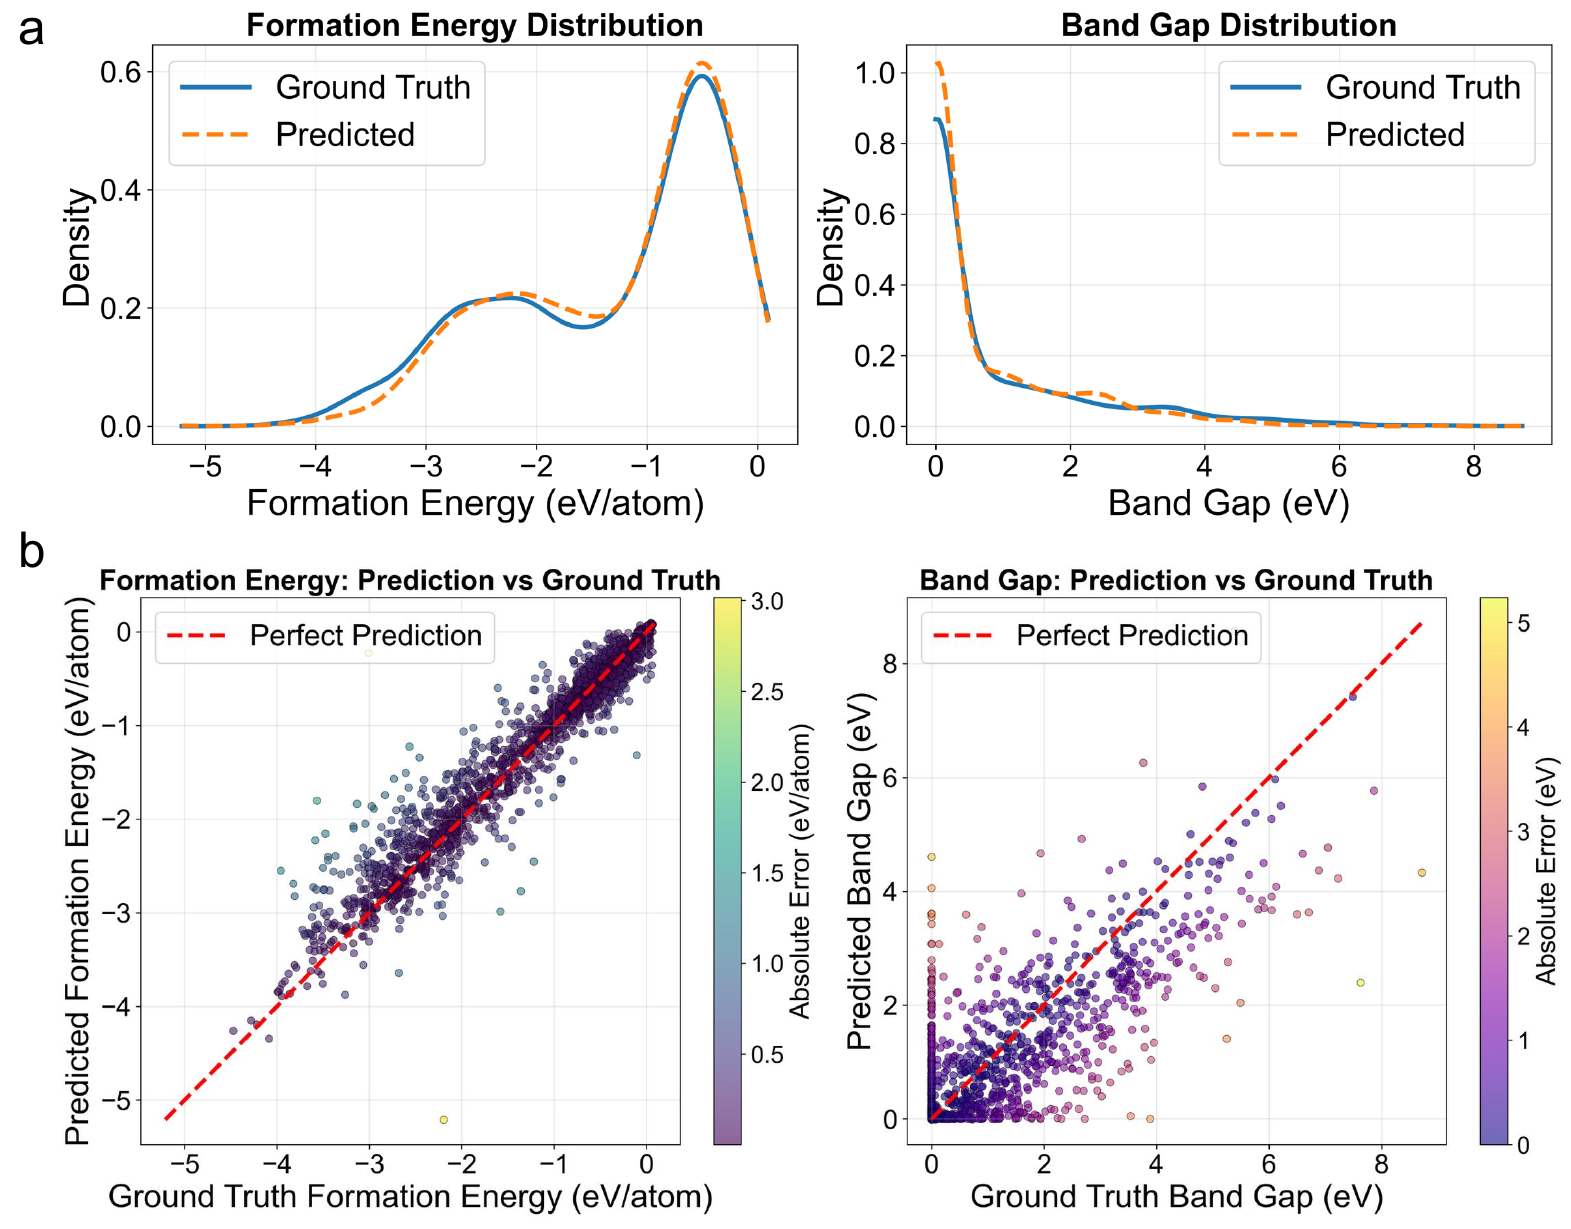
\includegraphics[width=\textwidth]{property.pdf}
\caption{\textbf{Generated crystals exhibit physically realistic properties.} \textbf{(a)} Kernel density estimates of formation energy (left) and band gap (right) for the MP-20 test set (solid) and the top 2,000 text-conditioned generated structures (dashed). The close overlap indicates that TFMat samples from thermodynamically and electronically plausible regions of crystal space. \textbf{(b)} Scatter plots of ground-truth versus CGCNN-predicted properties for 1,953 validated generated structures. Formation energy predictions (left) cluster tightly along the diagonal (Pearson $r = 0.92$, median absolute error 0.11~eV/atom), and band gap predictions (right) show reasonable agreement (Pearson $r = 0.78$, median absolute error 0.02~eV). Colour intensity indicates absolute prediction error. The red dashed line marks perfect prediction. High correlation and realistic distributions confirm that text conditioning preserves physical plausibility.}
\label{fig:property-validation}
\end{figure*}

\section*{Discussion}
The results clarify the role of text in crystal generation. TFMat does not simply make the model larger; it changes the conditional flow field through a semantic prior derived from text. This prior is most useful when the model must commit quickly, which is exactly the regime in which one-shot match rate matters. The strong gains over CrystalFlow across all three datasets show that the text signal sharpens the trajectory from noise to structure.

The comparison with TGDMat is also revealing. TGDMat (Long) remains extremely competitive, especially in one-shot RMSE on Perov-5 and MP-20 and in one-shot match rate on Carbon-24. Yet TFMat overtakes it on one-shot match rate for Perov-5 and MP-20, and on MP-20 with num\_eval=20 by a large margin. This suggests that a text-conditioned flow field can alter the global search behaviour of the generator in a way that repeated evolution alone does not fully reproduce.

At the same time, the MP-20 RMSE values show that retrieval and geometric refinement are not the same problem. The current formulation of TFMat is better at finding the correct structural basin than at achieving the very lowest final RMSE on MP-20. A natural next step is therefore to combine the present semantic conditioning strategy with a stronger refinement mechanism, such as more expressive multimodal fusion or a dedicated post-generation relaxer.

The de novo generation results extend this interpretation. In that setting, the main gain of TFMat is not a uniform increase in validity, but a marked improvement in distributional fidelity, especially for the element-count and density statistics of MP-20. The representative structures in Fig.~\ref{fig:mp20-dng-examples} are consistent with that reading: the model does not collapse to a single prototype family, but continues to sample chemically diverse crystals while preserving strong structural validity. Text guidance therefore appears to do more than nudge the model towards one target structure; it reshapes the regions of crystal space that the flow visits at the population level.

\section*{Conclusion}
TFMat introduces text-guided flow matching into crystal structure generation through a simple but effective conditioning mechanism. The method is defined by a continuous bridge from noise to crystal geometry, a text-derived semantic condition vector and guided Euler sampling. This design yields large gains over CrystalFlow in the single-sample regime and establishes the best MP-20 match rate under num\_eval=20 among the compared methods. In the de novo generation setting, TFMat further achieves the strongest MP-20 alignment on the number-of-elements and density statistics. The broader implication is that language can serve as a practical control interface for generative materials models, not merely as descriptive metadata but as an actionable prior over crystal structure space.

\section*{References}
Representative references should be finalized by the authors before submission. The present manuscript draft is based on the supplied repository, the provided evaluation summaries and the benchmark values transcribed from the user-provided figure.

\noindent\textbf{Acknowledgements}\\
Funding, institutional support and individual acknowledgements should be added by the authors before submission.

\noindent\textbf{Author contributions}\\
Author contribution statements should be added by the authors before submission.

\noindent\textbf{Competing interests}\\
The authors declare no competing interests.

\noindent\textbf{Data availability}\\
Data supporting the findings of this study are available from the corresponding author upon reasonable request.

\noindent\textbf{Code availability}\\
Code supporting the findings of this study is available from the corresponding author upon reasonable request.

\end{document}
